% Options for packages loaded elsewhere
% Options for packages loaded elsewhere
\PassOptionsToPackage{unicode}{hyperref}
\PassOptionsToPackage{hyphens}{url}
\PassOptionsToPackage{dvipsnames,svgnames,x11names}{xcolor}
%
\documentclass[
  letterpaper,
  DIV=11,
  numbers=noendperiod]{scrartcl}
\usepackage{xcolor}
\usepackage{amsmath,amssymb}
\setcounter{secnumdepth}{-\maxdimen} % remove section numbering
\usepackage{iftex}
\ifPDFTeX
  \usepackage[T1]{fontenc}
  \usepackage[utf8]{inputenc}
  \usepackage{textcomp} % provide euro and other symbols
\else % if luatex or xetex
  \usepackage{unicode-math} % this also loads fontspec
  \defaultfontfeatures{Scale=MatchLowercase}
  \defaultfontfeatures[\rmfamily]{Ligatures=TeX,Scale=1}
\fi
\usepackage{lmodern}
\ifPDFTeX\else
  % xetex/luatex font selection
\fi
% Use upquote if available, for straight quotes in verbatim environments
\IfFileExists{upquote.sty}{\usepackage{upquote}}{}
\IfFileExists{microtype.sty}{% use microtype if available
  \usepackage[]{microtype}
  \UseMicrotypeSet[protrusion]{basicmath} % disable protrusion for tt fonts
}{}
\makeatletter
\@ifundefined{KOMAClassName}{% if non-KOMA class
  \IfFileExists{parskip.sty}{%
    \usepackage{parskip}
  }{% else
    \setlength{\parindent}{0pt}
    \setlength{\parskip}{6pt plus 2pt minus 1pt}}
}{% if KOMA class
  \KOMAoptions{parskip=half}}
\makeatother
% Make \paragraph and \subparagraph free-standing
\makeatletter
\ifx\paragraph\undefined\else
  \let\oldparagraph\paragraph
  \renewcommand{\paragraph}{
    \@ifstar
      \xxxParagraphStar
      \xxxParagraphNoStar
  }
  \newcommand{\xxxParagraphStar}[1]{\oldparagraph*{#1}\mbox{}}
  \newcommand{\xxxParagraphNoStar}[1]{\oldparagraph{#1}\mbox{}}
\fi
\ifx\subparagraph\undefined\else
  \let\oldsubparagraph\subparagraph
  \renewcommand{\subparagraph}{
    \@ifstar
      \xxxSubParagraphStar
      \xxxSubParagraphNoStar
  }
  \newcommand{\xxxSubParagraphStar}[1]{\oldsubparagraph*{#1}\mbox{}}
  \newcommand{\xxxSubParagraphNoStar}[1]{\oldsubparagraph{#1}\mbox{}}
\fi
\makeatother


\usepackage{longtable,booktabs,array}
\usepackage{calc} % for calculating minipage widths
% Correct order of tables after \paragraph or \subparagraph
\usepackage{etoolbox}
\makeatletter
\patchcmd\longtable{\par}{\if@noskipsec\mbox{}\fi\par}{}{}
\makeatother
% Allow footnotes in longtable head/foot
\IfFileExists{footnotehyper.sty}{\usepackage{footnotehyper}}{\usepackage{footnote}}
\makesavenoteenv{longtable}
\usepackage{graphicx}
\makeatletter
\newsavebox\pandoc@box
\newcommand*\pandocbounded[1]{% scales image to fit in text height/width
  \sbox\pandoc@box{#1}%
  \Gscale@div\@tempa{\textheight}{\dimexpr\ht\pandoc@box+\dp\pandoc@box\relax}%
  \Gscale@div\@tempb{\linewidth}{\wd\pandoc@box}%
  \ifdim\@tempb\p@<\@tempa\p@\let\@tempa\@tempb\fi% select the smaller of both
  \ifdim\@tempa\p@<\p@\scalebox{\@tempa}{\usebox\pandoc@box}%
  \else\usebox{\pandoc@box}%
  \fi%
}
% Set default figure placement to htbp
\def\fps@figure{htbp}
\makeatother





\setlength{\emergencystretch}{3em} % prevent overfull lines

\providecommand{\tightlist}{%
  \setlength{\itemsep}{0pt}\setlength{\parskip}{0pt}}



 


\KOMAoption{captions}{tableheading}
\makeatletter
\@ifpackageloaded{caption}{}{\usepackage{caption}}
\AtBeginDocument{%
\ifdefined\contentsname
  \renewcommand*\contentsname{Table of contents}
\else
  \newcommand\contentsname{Table of contents}
\fi
\ifdefined\listfigurename
  \renewcommand*\listfigurename{List of Figures}
\else
  \newcommand\listfigurename{List of Figures}
\fi
\ifdefined\listtablename
  \renewcommand*\listtablename{List of Tables}
\else
  \newcommand\listtablename{List of Tables}
\fi
\ifdefined\figurename
  \renewcommand*\figurename{Figure}
\else
  \newcommand\figurename{Figure}
\fi
\ifdefined\tablename
  \renewcommand*\tablename{Table}
\else
  \newcommand\tablename{Table}
\fi
}
\@ifpackageloaded{float}{}{\usepackage{float}}
\floatstyle{ruled}
\@ifundefined{c@chapter}{\newfloat{codelisting}{h}{lop}}{\newfloat{codelisting}{h}{lop}[chapter]}
\floatname{codelisting}{Listing}
\newcommand*\listoflistings{\listof{codelisting}{List of Listings}}
\makeatother
\makeatletter
\makeatother
\makeatletter
\@ifpackageloaded{caption}{}{\usepackage{caption}}
\@ifpackageloaded{subcaption}{}{\usepackage{subcaption}}
\makeatother
\usepackage{bookmark}
\IfFileExists{xurl.sty}{\usepackage{xurl}}{} % add URL line breaks if available
\urlstyle{same}
\hypersetup{
  pdftitle={Pre-Lab 6},
  colorlinks=true,
  linkcolor={blue},
  filecolor={Maroon},
  citecolor={Blue},
  urlcolor={Blue},
  pdfcreator={LaTeX via pandoc}}


\title{Pre-Lab 6}
\author{}
\date{}
\begin{document}
\maketitle

\renewcommand*\contentsname{Table of contents}
{
\hypersetup{linkcolor=}
\setcounter{tocdepth}{3}
\tableofcontents
}

\subsection{Problem Statement: Task 1:}\label{problem-statement-task-1}

Figure~\ref{fig-task1} shows the intersection of a main highway with a
secondary access road. Vehicle-detection sensors are placed along lanes
C and D (main road) and lanes A and B (access road). These sensor
outputs are LOW (0) when no vehicle is present and HIGH (1) when a
vehicle is present. The intersection traffic light is to be controlled
according to the following logic:

\begin{enumerate}
\def\labelenumi{\arabic{enumi}.}
\tightlist
\item
  The east-west (E-W) traffic light will be green whenever both lanes C
  and D are occupied.
\item
  The E-W light will be green whenever either C or D is occupied but
  lanes A and B are not both occupied.
\item
  The north-south (N-S) light will be green whenever both lanes A and B
  are occupied but C and D are not both occupied.
\item
  The N-S light will also be green when either A or B is occupied while
  C and D are both vacant.
\item
  The E-W light will be green when no vehicles are present.
\end{enumerate}

Using the sensor outputs A, B, C, and D as inputs, design a logic
circuit to control the traffic light. There should be two outputs, N-S
and E-W, that go HIGH when the corresponding light is to be green.
Simplify the circuit as much as possible and show all steps.

\begin{figure}

\centering{

\includegraphics[width=3.125in,height=\textheight,keepaspectratio]{pre-lab-img/task1.png}

}

\caption{\label{fig-task1}}

\end{figure}%

Hints:

To design the logic circuit, follow the steps below:

\begin{enumerate}
\def\labelenumi{\arabic{enumi}.}
\tightlist
\item
  Design the truth table that satisfies the conditions in the problem.
\item
  Write the unsimplified Sum-of-Products expression for the output(s)
\item
  Complete Karnaugh map for the designed truth table.
\item
  Write the simplified expression for the output(s).
\item
  Draw the simplified circuit: Label all of the pin numbers on the
  diagram. Label all the ICs on the diagram.
\end{enumerate}

\subsection{\texorpdfstring{\textbf{Ans}:}{Ans:}}\label{ans}

1.

\begin{longtable}[]{@{}lllllll@{}}
\toprule\noalign{}
No. & A & B & C & D & E-W & N-S \\
\midrule\noalign{}
\endhead
\bottomrule\noalign{}
\endlastfoot
1 & 0 & 0 & 0 & 0 & 1 & 0 \\
2 & 0 & 0 & 0 & 1 & 1 & 0 \\
3 & 0 & 0 & 1 & 0 & 1 & 0 \\
4 & 0 & 0 & 1 & 1 & 1 & 0 \\
5 & 0 & 1 & 0 & 0 & 0 & 1 \\
6 & 0 & 1 & 0 & 1 & 1 & 0 \\
7 & 0 & 1 & 1 & 0 & 1 & 0 \\
8 & 0 & 1 & 1 & 1 & 1 & 0 \\
9 & 1 & 0 & 0 & 0 & 0 & 1 \\
10 & 1 & 0 & 0 & 1 & 1 & 0 \\
11 & 1 & 0 & 1 & 0 & 1 & 0 \\
12 & 1 & 0 & 1 & 1 & 1 & 0 \\
13 & 1 & 1 & 0 & 0 & 0 & 1 \\
14 & 1 & 1 & 0 & 1 & 0 & 1 \\
15 & 1 & 1 & 1 & 0 & 0 & 1 \\
16 & 1 & 1 & 1 & 1 & 1 & 0 \\
\end{longtable}

\newpage{}

2.

Unsimplified SOPs:

\(\text{E-W}\  = \overline{A}\ \,\overline{B}\ \,\overline{C}\ \,\overline{D}\  + \overline{A}\ \,\overline{B}\ \,\overline{C}\ D + \overline{A}\ \,\overline{B}\ C\overline{D}\  + \overline{A}\ \,\overline{B}\ CD + \overline{A}\ B\overline{C}\ D + \overline{A}\ BC\overline{D}\  + \overline{A}\ BCD + A\overline{B}\ \overline{C}\ D + A\overline{B}\ C\overline{D}\  + A\overline{B}\ CD + ABCD\)

\(\text{N-S}\  = \overline{A}\ B\overline{C}\ \,\overline{D}\  + A\overline{B}\ \,\overline{C}\ \,\overline{D}\  + AB\overline{C}\ \,\overline{D}\  + AB\overline{C}\ D + ABC\overline{D}\ \)

Karnaugh Maps:

3.

For \(\text{E-W}\):

\begin{figure}[H]

{\centering \pandocbounded{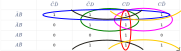
\includegraphics[keepaspectratio]{pre-lab_files/mediabag/ew-kmap.pdf}}

}

\caption{E-W Karnaugh map.}

\end{figure}%

For \(\text{N-S}\):

\begin{figure}[H]

{\centering \pandocbounded{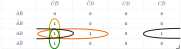
\includegraphics[keepaspectratio]{pre-lab_files/mediabag/ns-kmap.pdf}}

}

\caption{N-S Karnaugh map}

\end{figure}%

4.

Simplified expressions

\(\text{E-W} =  \overline{A}  \  \overline{B} + \overline{A}  \ D+ \overline{A}  \ C+ \overline{B}  \ D+ \overline{B}  \ C+C \ D\)

\(\text{N-S} = B \  \overline{C}  \  \overline{D} +A \  \overline{C}  \  \overline{D} +A \ B \  \overline{C} +A \ B \  \overline{D}\)

5.

\includegraphics[width=6.25in,height=\textheight,keepaspectratio]{./circuit.png}




\end{document}
